% Copyright (c) 2015 Daniele Masini - d.masini.it@gmail.com
% Copyright (c) 2016 Daniele Zambelli - daniele.zambelli@gmail.com

\section{Esercizi}

\subsection{Esercizi dei singoli paragrafi}

\begingroup
\hypersetup{linkcolor=black}
\subsubsection*{\ref{sect:poligoni_equivalenti} - 
\nameref{sect:poligoni_equivalenti}}
\endgroup

\begin{multicols}{2}

\begin{esercizio}
\label{ese:7.1}
Enunciate e dimostrate il teorema le cui ipotesi e tesi sono indicate 
di seguito.

\noindent Ipotesi: $AB\parallel DC$, $GH\perp AB$, $CJ\perp AB$, 
$AE\cong DE$, $CF\cong FB$.\\
\noindent Tesi: $ABCD\doteq GHJI$.\\

%
% \begin{inaccessibleblock}[Figura: TODO]
%  \begin{figure}[!htb]
% \noindent\centering% Copyright (c) 2015 Daniele Masini - d.masini.it@gmail.com

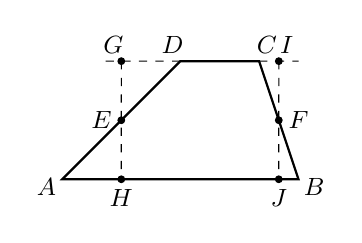
\begin{tikzpicture}[scale=1,font=\small]
\usetikzlibrary{calc}

\begin{scope}
\coordinate (a) at (0,0);
\coordinate (b) at (3,0);
\coordinate (c) at (2.5,1.5);
\coordinate (d) at (1.5,1.5);


\draw[thick] (a) node[shift={(-0.2,-0.1)}] {$A$} -- (b) node[shift={(0.2,-0.1)}] {$B$} -- (c) node[shift={(0.1,0.2)}] {$C$} -- (d) node[shift={(-0.1,0.2)}] {$D$} -- cycle;


\coordinate (e) at ($(a)!0.5!(d)$);
\coordinate (h) at ($(a)!(e)!(b)$);
\coordinate (f) at ($(b)!0.5!(c)$);
\coordinate (j) at ($(a)!(f)!(b)$);
\coordinate (g) at (intersection of h--e and c--d);
\coordinate (i) at (intersection of j--f and c--d);

\draw[dashed] (d) -- ($(d)!1.3!(g)$);
\draw[dashed] (c) -- ($(c)!2!(i)$);

\draw[dashed] (g) -- (h);
\draw[dashed] (i) -- (j);

\draw[fill] (e) circle (1.2pt) node[left] {$E$};
\draw[fill] (f) circle (1.2pt) node[right] {$F$};
\draw[fill] (g) circle (1.2pt) node[shift={(-0.1,0.2)}] {$G$};
\draw[fill] (i) circle (1.2pt) node[shift={(0.1,0.2)}] {$I$};
\draw[fill] (h) circle (1.2pt) node[below] {$H$};
\draw[fill] (j) circle (1.2pt) node[below] {$J$};

\end{scope}


\end{tikzpicture}

%	\caption{Esercizio~\ref{ese:7.1}}\label{fig:ese7.1}
%\end{figure}
% \end{inaccessibleblock}
\end{esercizio}
 
\begin{esercizio}
\label{ese:7.2}
Dai vertici $B$ e $C$ dell'ipotenusa di un triangolo rettangolo $ABC$ 
traccia le rette rispettivamente parallele ai cateti $AC$ e $AB$; sia 
$D$ il loro punto di intersezione. Dimostrare che $ABDC\doteq 2\cdot 
ABC$ e che $MNPQ\doteq 2\cdot ABC$ dove $MNPQ$ è il rettangolo avente 
un lato congruente all'ipotenusa $BC$ e l'altro lato congruente 
all'altezza $AH$ relativa all'ipotenusa.
\end{esercizio}

\begin{esercizio}
\label{ese:7.3}
Costruire un rettangolo equivalente ad un trapezio dato.
\end{esercizio}

\begin{esercizio}
\label{ese:7.4}
Dimostrare che la mediana relativa ad un lato di un triangolo divide 
il triangolo dato in due triangoli equivalenti.
\end{esercizio}

\begin{esercizio}
\label{ese:7.5}
Dimostrare che in un parallelogramma $ABCD$ sono equivalenti i 
quattro triangoli determinati dalle diagonali $AC$ e $BD$.
\end{esercizio}

\begin{esercizio}
\label{ese:7.6}
Assegnato il trapezio $ABCD$, detto $E$ il punto di intersezione 
delle diagonali $DB$ e $AC$, dimostrare che $DEA$ è equivalente a 
$BEC$.
\end{esercizio}

\begin{esercizio}
\label{ese:7.7}
Dimostra che le diagonali di un trapezio lo dividono in quattro 
triangoli due dei quali sono equiestesi.
\end{esercizio}

\begin{esercizio}
\label{ese:7.8}
Dimostra che due triangoli sono equiestesi se hanno due lati 
ordinatamente congruenti e gli angoli tra essi compresi supplementari.
\end{esercizio}

\begin{esercizio}
\label{ese:7.9}
Dimostra che un triangolo $ABC$ è diviso da una sua mediana in due 
triangoli equiestesi.
\end{esercizio}

\end{multicols}

\begingroup
\hypersetup{linkcolor=black}
\subsubsection*{\ref{sect:applicazioni_algebra} - 
\nameref{sect:applicazioni_algebra}}
\endgroup

\begin{multicols}{2}

\begin{esercizio}
\label{ese:7.10}
Sia $ABC$ un triangolo con $\overline{AB}=7$~cm, $\overline{BC}=5$~cm 
e $\overline{AC}=3$~cm. Condurre una parallela ad $AC$ che intersechi 
$AB$ in $D$ e $BC$ in $E$. Sapendo che $CE=BD$, trovare il perimetro 
del triangolo $BDE$.
\end{esercizio}

\begin{esercizio}
\label{ese:7.11}
Nel trapezio $ABCD$, le basi misurano 5~cm e 15~cm e l'area vale 
120~cm\textsuperscript{2}. Determina la distanza tra la base maggiore 
ed il punto di intersezione dei lati obliqui del trapezio.
\end{esercizio}

\begin{esercizio}
\label{ese:7.12}
Sia $ABC$ un triangolo rettangolo in $A$, con $AB=8a$. Da un punto 
$D$ di $AC$ si tracci la parallela ad $AB$ che incontri $BC$ in $E$; 
sia $DE=6a$. Sapendo che $CDE$ e $ABED$ sono isoperimetrici, trovare 
l'area di $ABC$.
\end{esercizio}

\begin{esercizio}
\label{ese:7.13}
Nel trapezio rettangolo $ABCD$ circoscritto ad una circonferenza  la 
base maggiore è $4/3$ dell'altezza ed il perimetro misura 48~cm. 
Trovare l'area del trapezio.
\end{esercizio}

\begin{esercizio}
\label{ese:7.14}
Sia $ABC$ un triangolo rettangolo con il cateto $AC = 32a$. Sapendo 
che $BC:AB=5:3$, trovare il perimetro del triangolo. Tracciare poi la 
parallela ad $AB$, che intersechi $CA$ in $D$ e $CB$ in $E$. Sapendo 
che $CD$ è medio proporzionale tra $CE$ ed $AB$, trovare l'area del 
trapezio $ABED$.
\end{esercizio}

\begin{esercizio}
\label{ese:7.15}
Sia $ABC$ un triangolo isoscele di base $BC=4$~cm e di area 
40~cm\textsuperscript{2}. Dopo aver trovato la misura dell'altezza 
$AH$ si tracci l'altezza $CK$ e la si prolunghi di un segmento $KD$ 
tale che l'angolo $H\widehat{A}D$ sia congruente ad uno degli angoli 
alla base. Dopo aver dimostrato che $C\widehat{A}D$ è retto, trovare 
il perimetro del triangolo $CAD$.
\end{esercizio}

\begin{esercizio}
\label{ese:7.16}
Due lati consecutivi di un parallelogramma misurano $2a$ e $4a$ e 
l'angolo tra essi compreso misura $60\grado$. Trovare la misura 
dell'area e delle diagonali.
\end{esercizio}

\begin{esercizio}
\label{ese:7.17}
Determinare perimetro ed area di un trapezio rettangolo circoscritto 
ad una circonferenza, sapendo che il lato obliquo è diviso dal punto 
di tangenza in due parti che misurano rispettivamente $4a$ e $9a$.
\end{esercizio}

\begin{esercizio}
\label{ese:7.18}
Determinare perimetro ed area di un triangolo isoscele, sapendo che 
la base misura $10a$ e che l'angolo adiacente ad uno degli angoli 
alla base misura $150\grado$.
\end{esercizio}

\begin{esercizio}
\label{ese:7.19}
Nel trapezio $ABCD$ la base maggiore, $AB$, misura 15~cm e la minore, 
$CD$, misura 5~cm. Prolungando i lati obliqui si ottiene un triangolo 
rettangolo. Trovare il perimetro del trapezio e del triangolo 
rettangolo $CDE$ sapendo che la differenza tra le due basi è uguale 
alla differenza tra il doppio di $BC$ e $AD$.
\end{esercizio}

\begin{esercizio}[Giochi di Archimede 2011]
\label{ese:7.20}
In un triangolo equilatero $ABC$ con lato di lunghezza 3~m, prendiamo 
i punti $D$, $E$ e $F$ sui lati $AC$, $AB$ e $BC$ rispettivamente, in 
modo che i segmenti $AD$ e $FC$ misurino 1~m e il segmento $DE$ sia 
perpendicolare ad $AC$. Quanto misura l'area del triangolo $DEF$?
\end{esercizio}

\begin{esercizio}
\label{ese:7.21}
\`E dato un trapezio isoscele avente un angolo di $45\grado$ e il 
lato obliquo che misura 2~cm. Trovare l'area sapendo che la base 
minore misura $\sqrt{3}$~cm.
\end{esercizio}

\begin{esercizio}
\label{ese:7.22}
Nella circonferenza di diametro $BD$ sono inscritti i triangoli $ABD$ 
e $BDC$, con $A$ e $C$ da parti opposte rispetto a $BD$. Sia $H$ la 
proiezione di $C$ su $BD$. Sapendo che $AB=16$~cm e che il rapporto 
tra $AD$ e $BD$ e tra $BH$ e $HD$ è $3/5$, trovare il perimetro di 
$ABCD$.
\end{esercizio}

\begin{esercizio}
\label{ese:7.23}
Il quadrato $ABCD$ ha il lato di 2~m; costruite sul lato $DC$ il 
triangolo isoscele $DEC$ di base $DC$ e avente 
$D\widehat{E}C=120\grado$; siano $F$ e $G$ i punti di intersezione 
delle rette $ED$ e $EC$ con la retta $AB$. Determinate la misura dei 
lati del triangolo $EFG$.
\end{esercizio}

\begin{esercizio}
\label{ese:7.24}
\`E dato il triangolo equilatero $ABC$; la semiretta $r$ di origine 
$B$ è interna all'angolo $ABC$ e lo divide in due parti di cui 
$ABP=45\grado$, $P0r\cap AC$. Sapendo che la distanza di $P$ dal lato 
$AB$ è di 2~m, calcolate il perimetro del triangolo equilatero dato.
\end{esercizio}

\begin{esercizio}
\label{ese:7.25}
Su ciascun lato del triangolo equilatero $ABC$ costruite un quadrato. 
Sapendo che l'altezza del triangolo equilatero misura $3\sqrt{3}$~m, 
determinate il perimetro e l'area dell'esagono che si forma 
congiungendo i vertici dei quadrati. Costruite il rettangolo 
equivalente all'esagono.
\end{esercizio}

\begin{esercizio}
\label{ese:7.26}
Nel trapezio rettangolo $ABCD$ di base maggiore $AB$, l'angolo acuto 
di vertice $B$ misura $45\grado$ e l'altezza è di 8~m. Sapendo che la 
base minore è $3/4$ dell'altezza, determinate perimetro e area del 
trapezio.
\end{esercizio}

\begin{esercizio}
\label{ese:7.27}
Nel parallelogramma $ABCD$ la diagonale minore $AC$ è perpendicolare 
al lato $BC$ e forma col lato $AB$ un angolo di $45\grado$. Sapendo 
che $AC=5$~m, calcolate il perimetro e l'area del parallelogramma.
\end{esercizio}

\begin{esercizio}
\label{ese:7.28}
Il trapezio $ABCD$ di base maggiore $AB$, ha $\widehat{A}=45\grado$ e 
$\widehat{B}=60\grado$; sapendo che la base minore è uguale 
all'altezza che misura 12~cm, determinate perimetro e area del 
trapezio.
\end{esercizio}

\begin{esercizio}
\label{ese:7.29}
Il quadrilatero $ABCD$ è spezzato dalla diagonale $AC$ nel triangolo 
rettangolo isoscele $ABC$ retto in $B$ e nel triangolo $ADC$ isoscele 
su $AC$, avente l'altezza $DH$ doppia della base. Sapendo che 
$AB=5$~m, calcolate il perimetro e l'area del quadrilatero.
\end{esercizio}

\begin{esercizio}
\label{ese:7.30}
Il triangolo isoscele $ABC$ ha l'angolo in $A$ opposto alla base $BC$ 
di $120\grado$ ed è circoscritto ad una circonferenza di raggio 
$OH=\sqrt{6}$~m; calcolate perimetro e area del triangolo dato.
\end{esercizio}

\begin{esercizio}
\label{ese:7.31}
Nel triangolo $ABC$ l'angolo in $A$ misura $60\grado$ e sia $AE$ la 
sua bisettrice ($E$ su $BC$). Sapendo che $AE=8$~m, determinate la 
misura delle distanze $EH$ ed $EK$ del punto $E$ rispettivamente dai 
lati $AB$ e $AC$ e il perimetro del quadrilatero $AHEK$. \`E vero che 
tale quadrilatero è equivalente al triangolo equilatero di lato 8~m? 
\`E vero che tale quadrilatero può essere inscritto in una 
circonferenza? Se la risposta è affermativa stabilite il suo centro e 
determinate la misura di detta circonferenza.
\end{esercizio}

\begin{esercizio}
\label{ese:7.32}
Nel trapezio rettangolo $ABCD$ la base minore è metà dell'altezza. 
Determinate perimetro e area in funzione della misura $x$ della base 
minore nei casi in cui l'angolo acuto del trapezio è di
\begin{enumeratea}
\item $45\grado$;
\item $30\grado$;
\item $60\grado$.
\end{enumeratea}
\end{esercizio}

\begin{esercizio}
\label{ese:7.33}
Il triangolo $ABC$ è rettangolo e l'angolo di vertice $C$ misura 
$30\grado$; detta $AP$ la bisettrice dell'angolo retto, con $P$ su 
$BC$, e sapendo che $\overline{AP}=a$, determinate, in funzione di 
$a$, perimetro e area del triangolo dato.
\end{esercizio}

\begin{esercizio}
\label{ese:7.34}
Il segmento $AC$ è la diagonale del quadrilatero $ABCD$ avente 
$A\widehat{B}C=C\widehat{A}D=90\grado$ e 
$B\widehat{C}A=A\widehat{D}C=60\grado$. \`E vero che $ABCD$ è un 
trapezio rettangolo? Calcolate perimetro e area del quadrilatero 
sapendo che $\overline{AC}=2a$.
\end{esercizio}

\begin{esercizio}
\label{ese:7.35}
Il quadrato $ABCD$ ha i suoi vertici sui lati del triangolo 
equilatero $HKL$ ($A$ e $B$ appartengono a $KL$, $C$ a $HL$ e $D$ a 
$HK$); sapendo che $\overline{AB}=3a$, calcolate il perimetro e l'area 
del triangolo equilatero.
\end{esercizio}

\begin{esercizio}
\label{ese:7.36}
In un parallelogramma di area 12~m\textsuperscript{2}, le lunghezze 
di due lati consecutivi sono una il doppio dell'altra e uno degli 
angoli interni misura $60\grado$. Determina la lunghezza delle 
diagonali.
\end{esercizio}

\begin{esercizio}
\label{ese:7.37}
Nel triangolo $ABC$ di altezza $CH=8$~m, determina a quale distanza 
da $C$ si deve condurre una parallela al lato $AB$ in modo che il 
triangolo ottenuto sia equivalente alla metà di $ABC$.
\end{esercizio}

\begin{esercizio}
\label{ese:7.38}
La base di un rettangolo è più lunga di 8~cm dell'altezza ed è più 
corta di 10~cm della diagonale. Calcola perimetro ed area del 
rettangolo. 			
\end{esercizio}

\begin{esercizio}
\label{ese:7.39}
In un triangolo equilatero $ABC$ di lato $l$ individua sul lato $AB$ 
un punto $P$ tale che detti $H$ e $K$ i piedi delle perpendicolari 
condotte da $P$ ai lati $AC$ e $BC$ risulti 
$\overline{PH}^2+\overline{PK}^2=\overline{PC}^2+\np{12,67}$
\end{esercizio}

\begin{esercizio}
\label{ese:7.40}
Un triangolo equilatero e un quadrato hanno lo stesso perimetro. 
Quanto vale il rapporto tra le aree delle due figure?
\end{esercizio}

\begin{esercizio}
\label{ese:7.41}
In un triangolo rettangolo $ABC$, retto in $A$, si tracci una 
parallela $DE$ al cateto $AB$. Sapendo che l'area di $DEC$ è i $3/4$ 
di quella di $ABC$ e che $\overline{AC}$ misura 1~m, quanto misura 
$\overline{DC}$?
\end{esercizio}

\begin{esercizio}
\label{ese:7.42}
Dato il quadrato $ABCD$ con $M$ punto medio di $AB$ ed $N$ punto 
medio di $CD$, tracciare i segmenti $AN$, $BN$, $DM$ e $CM$. Siano 
$P$ l'intersezione di $AN$ con $DM$ e $Q$ l'intersezione di $BN$ e 
$CM$. Che figura è $MQNP$? Quanti triangoli ci sono nella figura? 
Calcolare l'area di $MQNP$ e l'area di uno dei triangoli ottusangoli, 
sapendo che il lato del quadrato è 12~cm.
\end{esercizio}

\begin{esercizio}
\label{ese:7.43}
Disegna un rombo con la diagonale minore lunga 6~cm e la diagonale 
maggiore 8~cm. Costruisci su ciascun lato del rombo un quadrato. 
Unisci i vertici liberi dei quadrati formando un ottagono. Calcolane 
l'area. Calcola anche l'area dei quattro triangoli che si sono 
formati. Calcola inoltre la misura degli angoli interni dell'ottagono.
\end{esercizio}

\begin{esercizio}
\label{ese:7.44}
Disegna un quadrato $ABCD$ e sul lato $AB$ poni i punti $M$ ed $N$ in 
modo che $AM\cong MN\cong NB$. Che figura è $MNCD$? Calcola il 
rapporto tra l'area di $MNCD$ e quella di $ABCD$. Calcola il 
perimetro di $MNCD$ sapendo che l'area del quadrato è 
10~cm\textsuperscript{2}.
\end{esercizio}

\begin{esercizio}
\label{ese:7.45}
Disegna un triangolo isoscele $ABC$ di base $AC=40$~mm e lato obliquo 
$AB=52$~mm. Costruisci sulla base $AC$ il triangolo $ACD$ di area 
doppia di $ABC$ e determina il perimetro del quadrilatero $ABCD$. Di 
che figura si tratta?
\end{esercizio}

\begin{esercizio}
\label{ese:7.46}
Il parallelogramma $ABCD$ ha la base $AB$ lunga 12~cm e l'altezza di 
6~cm. Disegna su $AB$ un punto $H$ e su $CD$ un punto $K$ tali che 
$DK=BH=3$~cm. Considera i due quadrilateri in cui il parallelogramma 
rimane diviso dal segmento $HK$: che quadrilateri sono? Calcolane 
l'area. Calcola inoltre il rapporto tra l'area di $HBCD$ e quella di 
$ABCD$.
\end{esercizio}

\begin{esercizio}
\label{ese:7.47}
Calcola l'altezza del rombo avente le diagonali di 36~cm e 48~cm. 
Calcola l'area del trapezio equivalente al rombo, sapendo che 
l'altezza del trapezio è di 24~cm e che la base maggiore è il doppio 
di quella minore.
\end{esercizio}

\begin{esercizio}
\label{ese:7.48}
Il rettangolo $R$ ha base $AB = 9$~cm e l'altezza $BC$ è i $4/3$ di 
$AB$. Calcola il perimetro e l'area di $R$. Disegna il 
parallelogramma $P$ equivalente al rettangolo $R$ e avente la base 
congruente alla diagonale del rettangolo. Calcola l'altezza di $P$.
\end{esercizio}

\begin{esercizio}
\label{ese:7.49}
Calcola l'area del parallelogramma $P$ di base \np{4,5}~cm e altezza 
2~cm e con il lato obliquo che è $5/4$ dell'altezza. Disegna la 
diagonale $AC$ e traccia l'altezza relativa ad $AB$ del triangolo 
$ABC$. Calcola l'area del triangolo $ABC$.
\end{esercizio}

\begin{esercizio}
\label{ese:7.50}
I lati del triangolo $ABC$ hanno le seguenti misure $AB=21$~cm, 
$BC=20$~cm e $AC=13$~cm; calcola l'area del parallelogramma 
$A'B'C'D'$ di base $AB\cong A'B'$, lato $AC\cong A'C'$ e diagonale 
$B'C'\cong BC$ (ricorda la formula di Erone).
\end{esercizio}

\begin{esercizio}
\label{ese:7.51}
Dato il rombo $ABCD$, avente perimetro di 10~cm e la diagonale 
maggiore di 4~cm, calcola la misura della diagonale minore, l'area 
del rombo e la sua altezza. Considera un triangolo isoscele 
equivalente al rombo e avente la sua stessa altezza. Calcolane la 
misura di ciascun lato.
\end{esercizio}

\begin{esercizio}
\label{ese:7.52}
Un rombo ha l'area di 336~cm\textsuperscript{2}, una diagonale uguale 
alla base di un triangolo di altezza \np{20,2}~cm e area di 
\np{141,4}~cm\textsuperscript{2}. Determina il perimetro del rombo.
\end{esercizio}

\begin{esercizio}
\label{ese:7.53}
Determina l'area del quadrato formato dai 4 vertici liberi di 4 
triangoli equilateri costruiti sui lati di un quadrato di lato 3~cm.
\end{esercizio}

\begin{esercizio}
\label{ese:7.54}
Determina l'area del rombo intersezione di due triangoli equilateri 
costruiti sui lati opposti di un quadrato di lato 10~cm e aventi il 
vertice che cade internamente al quadrato.
\end{esercizio}

\begin{esercizio}
\label{ese:7.55}
Determina le misure degli angoli del triangolo $AED$ formato 
disegnando le diagonali $EA$ e $AD$ di un esagono regolare $ABCDEF$.
\end{esercizio}

\begin{esercizio}
\label{ese:7.56}
Determina le misure degli angoli del triangolo $AEC$ formato 
disegnando le diagonali $EA$ ed $EC$ di un ottagono regolare 
$ABCDEFGH$.
\end{esercizio}

\begin{esercizio}
\label{ese:7.57}
Determina le misure degli angoli del triangolo $AFC$ formato 
disegnando le diagonali $AF$ e $FC$ di un ottagono regolare 
$ABCDEFGH$.
\end{esercizio}

\begin{esercizio}
\label{ese:7.58}
La differenza tra le diagonali di un rombo è 7~cm e una è $5/12$ 
dell'altra. Determina l'area di un triangolo isoscele il cui 
perimetro supera di 6~cm quello del rombo e la cui base è 8~cm.
\end{esercizio}

\begin{esercizio}
\label{ese:7.59}
Determinare l'area di un quadrilatero con le diagonali perpendicolari 
sapendo che l'una è $5/8$ dell'altra e che la loro somma è 39~cm.
\end{esercizio}

\begin{esercizio}
\label{ese:7.60}
Determinare la misura degli angoli di un parallelogramma sapendo che 
uno degli angoli alla base è $2/7$ di quello adiacente.
\end{esercizio}

\begin{esercizio}
\label{ese:7.61}
In un quadrilatero un angolo è $93\grado8'42''$. Determinare 
l'ampiezza di ciascuno degli altri tre angoli sapendo che il secondo 
è $2/7$ del terzo e il terzo è $4/5$ del quarto.
\end{esercizio}

\begin{esercizio}
\label{ese:7.62}
Le dimensioni $a$ e $b$ di un rettangolo sono $a=\frac{3}{5}b$, il 
perimetro è 192~cm. Calcolane l'area.
\end{esercizio}

\begin{esercizio}
\label{ese:7.63}
In un rombo la differenza fra le diagonali è 8~cm e una diagonale è i 
$4/3$ dell'altra. Calcola area e perimetro del rombo.
\end{esercizio}

\begin{esercizio}
\label{ese:7.64}
In un rombo la somma delle diagonali misura 196~cm, un quarto della 
misura della diagonale maggiore supera di 4~cm la misura della 
diagonale minore. Trova perimetro, area e altezza del rombo.
\end{esercizio}

\begin{esercizio}
\label{ese:7.65}
In un trapezio rettangolo l'altezza è quadrupla della base minore e 
il lato obliquo è i $5/4$ dell'altezza. Determina l'area del trapezio 
sapendo che il suo perimetro è 70~cm.
\end{esercizio}

\begin{esercizio}
\label{ese:7.66}
Il perimetro di un trapezio isoscele misura 124~cm e ciascun lato 
obliquo è lungo 30~cm. Determinane l'area e la misura della diagonale 
sapendo che una sua base è $7/25$ dell'altra.
\end{esercizio}

\begin{esercizio}
\label{ese:7.67}
Determina l'area di un rettangolo sapendo che la misura della sua 
diagonale supera di 8~cm quella dell'altezza e che la differenza fra 
i $20/41$ della diagonale ed i $2/3$ dell'altezza è uguale ai $14/9$ 
della stessa altezza.
\end{esercizio}

\begin{esercizio}
\label{ese:7.68}
Il perimetro di un rettangolo misura 170~cm e l'altezza è $5/12$ 
della base. Trovare area e diagonale del rettangolo.
\end{esercizio}

\begin{esercizio}
\label{ese:7.69}
Il perimetro di un rettangolo misura 29~cm ed i $2/11$ della sua 
altezza sono uguali a $1/9$ della base. Trovare l'area del rettangolo.
\end{esercizio}

\begin{esercizio}
\label{ese:7.70}
In un trapezio isoscele $ABCD$ avente la base maggiore $AB$, le 
diagonali sono fra loro perpendicolari e si intersecano in un punto 
$P$ che divide ogni diagonale in due parti con rapporto $5/12$. 
Calcola perimetro e area del trapezio, sapendo che la diagonale 
misura 68~cm.
\end{esercizio}

\begin{esercizio}
\label{ese:7.71}
Un triangolo rettangolo ha ipotenusa 50~cm e un cateto 48~cm. Dal 
punto medio dell'ipotenusa tracciare la parallela al cateto minore. 
Determinare l'area di ciascuna delle due parti in cui è suddiviso il 
triangolo.
\end{esercizio}

\begin{esercizio}
\label{ese:7.72}
In un triangolo l'altezza è 18~cm; se conducendo una parallela alla 
base, si divide il triangolo in due parti la cui superficie è in 
rapporto $16/25$, a quale distanza dal vertice è stata condotta la 
parallela?
\end{esercizio}

\begin{esercizio}
\label{ese:7.73}
Il triangolo $ABC$ ha base 14~cm e altezza 6~cm. Disegna la mediana 
$CM$ e calcola l'area dei triangoli $AMC$ e $MBC$. Come sono i 
triangoli?
\end{esercizio}

\begin{esercizio}
\label{ese:7.74}
La mediana di un triangolo è 12~cm. Determinare la misura di ciascuna 
delle parti in cui il baricentro divide la mediana.
\end{esercizio}

\begin{esercizio}
\label{ese:7.75}
Determinare la misura di una mediana $AM$ sapendo che $BM=8$~cm, dove 
$B$ è il baricentro del triangolo.
\end{esercizio}

\begin{esercizio}
\label{ese:7.76}
Determina la misura $BM$ del segmento appartenente alla mediana $AM$ 
in un triangolo equilatero $ABC$, avendo indicato con $B$ il 
baricentro. 
\end{esercizio}

\begin{esercizio}
\label{ese:7.77}
Determina il perimetro di un triangolo rettangolo sapendo che 
l'altezza relativa all'ipotenusa è 8~cm e che la proiezione di un 
cateto sull'ipotenusa è $4/3$ dell'altezza data.
\end{esercizio}

\begin{esercizio}
\label{ese:7.78}
Determina la misura delle tre altezze del triangolo che ha i lati di 
20~cm, 40~cm, 30~cm. (Suggerimento: Puoi ricorrere alla formula di 
Erone).
\end{esercizio}

\begin{esercizio}
\label{ese:7.79}
Il piede dell'altezza $CH$ di un triangolo $ABC$ divide la base $AB$ 
di 46~cm in due parti tali che $AH=\dfrac{9}{14}HB$; calcola l'area 
dei due triangoli $ACH$ e $BCH$, sapendo che $AC=24$~cm.
\end{esercizio}

\begin{esercizio}
\label{ese:7.80}
Trova il perimetro di un triangolo isoscele sapendo che la base è 
$2/3$ dell'altezza e che l'area è 24~cm\textsuperscript{2}.
\end{esercizio}

\begin{esercizio}
\label{ese:7.81}
Trova il perimetro di un triangolo isoscele sapendo che la base è 
$3/5$ dell'altezza e che l'area è 24~cm\textsuperscript{2}.
\end{esercizio}

\begin{esercizio}
\label{ese:7.82}
I lati del triangolo $ABC$ hanno le misure seguenti $AB=63$~cm, 
$BC=60$~cm e $AC=39$~cm; determina le misure delle tre relative 
altezze.
\end{esercizio}

\begin{esercizio}
\label{ese:7.83}
Determinare la misura di ciascun lato e l'area del triangolo isoscele 
avente il perimetro di 700~m, sapendo che la base e il lato obliquo 
sono in rapporto $\frac{16}{17}$.
\end{esercizio}

\begin{esercizio}
\label{ese:7.84}
Un trapezio rettangolo $ABCD$ è circoscritto ad una semicirconferenza 
con il centro $O$ sulla sua base maggiore $AB$ e raggio di misura 
6~cm. Siano $S$ e $T$ i punti in cui tale semicirconferenza tange 
rispettivamente il lato obliquo $BC$ e la base minore $CD$. Sapendo 
che $AB$ misura 16~cm, calcolare le misure degli altri lati del 
trapezio. (Tracciare $OC$, $OS$, $OT$ e dimostrare che $OB$ è 
congruente a \ldots{}).
\end{esercizio}

\begin{esercizio}
\label{ese:7.85}
Calcolare perimetro e area di un triangolo isoscele circoscritto a 
una semicirconferenza con il centro sulla sua base, sapendo che la 
base è i $3/2$ della relativa altezza e che il raggio della 
semicirconferenza misura 12~cm.
\end{esercizio}

\begin{esercizio}
\label{ese:7.86}
Data una circonferenza di centro $O$, si consideri un punto $C$ 
esterno ad essa da cui si traccino le tangenti alla circonferenza 
stessa indicando con $A$ e $B$ i punti di tangenza. Sapendo che il 
segmento $AB$ misura 12~cm e che l'angolo $A\widehat{C}B$ ha ampiezza 
$60\grado$, calcolare il perimetro e l'area del quadrilatero $OACB$. 
Indicato poi con $E$ il punto in cui la retta $OB$ incontra la retta 
$AC$, calcolare il perimetro del triangolo $BCD$.
\end{esercizio}

\begin{esercizio}
\label{ese:7.87}
In un trapezio rettangolo, l'angolo che il lato obliquo forma con la 
base maggiore ha ampiezza $60\grado$ e la diagonale maggiore dimezza 
tale angolo; sapendo che la base minore misura 4~cm,  calcolare il 
perimetro del trapezio.
\end{esercizio}

\begin{esercizio}
\label{ese:7.88}
In un rombo $ABCD$ ciascun lato misura 12~cm e l'angolo in $B$ ha 
ampiezza $120\grado$. Prendere sui lati $AB$, $BC$, $CD$ e $AD$ del 
rombo rispettivamente i punti $P$, $Q$, $S$ e $T$ in modo che i 
segmenti $AP$, $BQ$, $CS$ e $DT$ misurino 2~cm ciascuno. Calcolare il 
perimetro e l'area del quadrilatero $PQST$, dopo aver dimostrato che 
esso è un parallelogramma. (Tracciare da $T$ il segmento 
perpendicolare ad $AB$ e osservare i vari triangoli \ldots{}, 
analogamente tracciare poi da $P$ il segmento perpendicolare alla 
retta \ldots{}).  
\end{esercizio}

\begin{esercizio}
\label{ese:7.89}
Sul lato $AB$ di un triangolo equilatero $ABC$ avente area uguale a 
$25\sqrt{3}$~cm\textsuperscript{2}, si prenda il punto $P$ in modo 
che $AP$ misuri 4~cm; si tracci il segmento $PQ$ parallelo a $BC$ (con 
$Q$ appartenente ad $AC$) e lo si prolunghi di un segmento $QE$ 
congruente a $PQ$. Dopo aver dimostrato che il triangolo $APE$ è 
rettangolo, calcolare perimetro ed area del quadrilatero $CEPH$, 
essendo $H$ il piede dell'altezza del triangolo $ABC$ relativa ad 
$AB$.
\end{esercizio}

\begin{esercizio}
\label{ese:7.90}
Data una semicirconferenza di centro $O$ e diametro $AB$ di misura 
$2r$, si tracci la corda $AC$ che forma con $AB$ un angolo di 
$30\grado$; si tracci quindi la tangente in $C$ alla 
semicirconferenza indicando con $D$ il punto in cui tale tangente 
incontra la retta $AB$ e con $E$ la proiezione ortogonale di $B$ sulla 
tangente stessa. Calcolare le misure dei segmenti $BC$, $CD$, $BE$, 
$CE$, $AE$. (Tracciare anche $CO$ \ldots{} osservare i vari angoli; 
per calcolare la misura di $AE$ tracciare la distanza di \ldots{} 
dalla retta \ldots{}).
\end{esercizio}

\begin{esercizio}
\label{ese:7.91}
Determina area e perimetro del quadrilatero $ABCD$ di coordinate 
$A(-1;7)$, $B(6;9/2)$, $C(4;-3)$ e $D(-4;3)$.
\end{esercizio}

\begin{esercizio}
\label{ese:7.92}
Determina area a perimetro del quadrilatero $ABCD$ di coordinate 
$A(0;3)$, $B(3;6)$, $C(6;3)$ e $D(-4;3)$. Che quadrilatero è?
\end{esercizio}

\begin{esercizio}
\label{ese:7.93}
Determina l'area del quadrilatero $ABCD$ di coordinate $A(-8;5)$, 
$B(-2;11)$, $C(2;12)$ e $D(4;3)$.
\end{esercizio}

\begin{esercizio}
\label{ese:7.94}
Determina il quarto vertice $D$ del trapezio $ABCD$ di area $9$, 
sapendo che $A(-1;2)$, $B(5;2)$ e $C(3;4)$.
\end{esercizio}

\begin{esercizio}
\label{ese:7.95}
Determina il quarto vertice $D$ del parallelogramma $ABCD$ con 
$A(-3;-1)$, $B(4;1)$ e $C(3;4)$.
\end{esercizio}

\begin{esercizio}
\label{ese:7.96}
Verifica che il trapezio di vertici $A(-1;-1)$, $B(3;-2)$, 
$C\left(3;\frac{1}{2}\right)$ e $D\left(0;\frac{5}{2}\right)$ non è 
rettangolo. Calcola l'intersezione $E$ dei prolungamenti dei lati 
obliqui $BC$ e $AD$. Calcola inoltre il rapporto tra le aree dei 
triangoli $ABE$ e $CDE$.
\end{esercizio}

\begin{esercizio}
\label{ese:7.97}
Verifica che il quadrilatero di vertici $A(-2;-3)$, $B(3;-2)$, 
$C(4;1)$ e $D(0;3)$ è un trapezio e calcolane l'altezza.
\end{esercizio}

\begin{esercizio}
\label{ese:7.98}
Verifica che il quadrilatero di vertici $A(-4;1)$, $B(5;-2)$, 
$C(3;2)$ e $D(0;3)$ è un trapezio isoscele. Calcola l'intersezione $E$ 
dei prolungamenti dei lati obliqui $BC$ e $AD$. Calcola inoltre il 
rapporto tra le aree dei triangoli $ABE$ e $CDE$.
\end{esercizio}

\begin{esercizio}[Giochi di Archimede 2011]
\label{ese:7.99}
Nel quadrilatero $ABCD$ le diagonali sono ortogonali tra loro e gli 
angoli in $B$ e in $D$ sono retti. Inoltre $AB=AD=20$~cm e 
$BC=CD=30$~cm. Calcolare il raggio della circonferenza inscritta in 
$ABCD$.
\end{esercizio}

\begin{esercizio}[Giochi di Archimede 2003]
\label{ese:7.100}
Sia dato un quadrato $ABCD$ di lato unitario e sia $P$ un punto 
interno ad esso tale che l'angolo $A\widehat{P}B$ misuri $75\grado$. 
Quanto vale la somma delle aree dei triangoli $ABP$ e $CDP$? 
\end{esercizio}

\begin{esercizio}[Giochi di Archimede 2003]
\label{ese:7.101}
Un parallelogramma di lati 1 e 2 ha un angolo di $60\grado$. Quanto 
misura la sua diagonale minore?   
\end{esercizio}

\begin{esercizio}[Giochi di Archimede 2007]
\label{ese:7.102}
In un triangolo $ABC$ scegliamo un punto $D$ su $AB$ e un punto $E$ 
su $AC$ in modo che la lunghezza di $AD$ sia un terzo di quella di 
$AB$ e la lunghezza di $AE$ sia un terzo di quella di $AC$. Sapendo 
che l'area del triangolo $ADE$ è 5~m\textsuperscript{2}, determinare 
l'area del quadrilatero $BCED$.
\end{esercizio}

\begin{esercizio}[Giochi di Archimede 2007]
\label{ese:7.103}
Il quadrato $ABCD$ ha il lato lungo 3~m. Il segmento $EF$ è lungo 1~m 
ed è parallelo ad $AB$. Quanto vale l'area dell'esagono $ABFCDE$?
\end{esercizio}

%
% \begin{inaccessibleblock}[Figura: TODO]
%  \begin{figure}[!htb]
% 	\centering% Copyright (c) 2015 Daniele Masini - d.masini.it@gmail.com

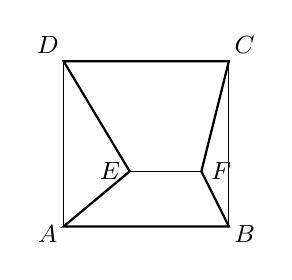
\begin{tikzpicture}[scale=0.7,font=\small]
\usetikzlibrary{calc}

\begin{scope}
\coordinate (a) at (0,0);
\coordinate (b) at (3,0);
\coordinate (c) at (3,3);
\coordinate (d) at (0,3);
\coordinate (e) at (1.2,1);
\coordinate (f) at (2.5,1);

\draw[thick] (a) node[shift={(-0.2,-0.1)}] {$A$} -- (b) node[shift={(0.2,-0.1)}] {$B$} -- (f) node[shift={(0.25,0)}] {$F$} -- (c) node[shift={(0.2,0.2)}] {$C$} -- (d) node[shift={(-0.2,0.2)}] {$D$} -- (e) node[shift={(-0.25,0)}] {$E$} -- cycle;
\draw (a) -- (d);
\draw (b) -- (c);
\draw (e) -- (f);

\end{scope}


\end{tikzpicture}

%	\caption{Esercizio~\ref{ese:7.104}}\label{fig:ese7.104}
%\end{figure}
% \end{inaccessibleblock}

\begin{esercizio}[Giochi di Archimede 2007]
\label{ese:7.104}
$ABCD$ è un quadrato avente la diagonale lunga 2~cm e $AEC$ è 
equilatero. Quanto vale l'area del quadrilatero $AECB$?
\end{esercizio}

%
% \begin{inaccessibleblock}[Figura: TODO]
%  \begin{figure}[!htb]
% 	\centering% Copyright (c) 2015 Daniele Masini - d.masini.it@gmail.com

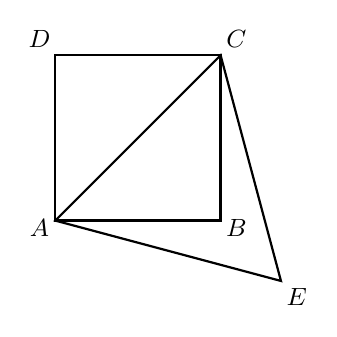
\begin{tikzpicture}[scale=0.7,font=\small]
\usetikzlibrary{calc, intersections}

\begin{scope}
\clip (-0.5,-1.6) rectangle (4.6,3.5);
\coordinate (a) at (0,0);
\coordinate (b) at (3,0);
\coordinate (c) at (3,3);
\coordinate (d) at (0,3);

\path[name path = Circle1] (a) let \p1 = ($(c)-(a)$) in circle ({veclen(\x1,\y1)});
\path[name path = Circle2] (c) let \p1 = ($(a)-(c)$) in circle ({veclen(\x1,\y1)});
\path [name intersections={of=Circle1 and Circle2}];
\path (intersection-2) coordinate (e) node[shift={(0.2,-0.2)}] {$E$};

\draw[thick] (a) node[shift={(-0.2,-0.1)}] {$A$} -- (b) node[shift={(0.2,-0.1)}] {$B$} -- (c) node[shift={(0.2,0.2)}] {$C$} -- (d) node[shift={(-0.2,0.2)}] {$D$} -- cycle;
\draw[thick] (a) -- (c) -- (e) -- cycle;

\end{scope}


\end{tikzpicture}

%	\caption{Esercizio~\ref{ese:7.105}}\label{fig:ese7.105}
%\end{figure}
% \end{inaccessibleblock}

\begin{esercizio}[Giochi d'Autunno 2010]
\label{ese:7.105}
Da un quadrato di lato 10~cm si tagliano i quattro angoli in modo da 
ottenere un ottagono regolare. Quanto è lungo il lato dell'ottagono?
\end{esercizio}

%
% \begin{inaccessibleblock}[Figura: TODO]
%  \begin{figure}[!htb]
% 	\centering% Copyright (c) 2015 Daniele Masini - d.masini.it@gmail.com

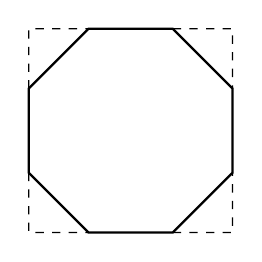
\begin{tikzpicture}[scale=0.7,font=\small]
\usetikzlibrary{calc}
\pgfmathsetmacro{\lati}{8}
\pgfmathsetmacro{\angoloc}{360/\lati}

\begin{scope}[rotate={\angoloc/2-90}]
\coordinate (o) at (0,0);

\foreach \x/\y in {0/A,1/B,2/C,3/D,4/E,5/F,6/G,7/H}
{
	\path +({\x*\angoloc}:2) coordinate (\y) -- ({(\x+1)*\angoloc}:2);
}
\draw[thick] (A) -- (B) -- (C) -- (D) -- (E) -- (F) -- (G) -- (H) -- cycle; 

\end{scope}

\coordinate (ef) at (intersection of D--E and G--F);
\coordinate (cd) at (intersection of D--E and C--B);
\coordinate (ab) at (intersection of C--B and A--H);
\coordinate (gh) at (intersection of A--H and F--G);

\draw[dashed] (F) -- (ef) -- (E);
\draw[dashed] (D) -- (cd) -- (C);
\draw[dashed] (A) -- (ab) -- (B);
\draw[dashed] (G) -- (gh) -- (H);

\end{tikzpicture}

%	\caption{Esercizio~\ref{ese:7.106}}\label{fig:ese7.106}
%\end{figure}
% \end{inaccessibleblock}

\begin{esercizio}[Giochi di Archimede 2006]
\label{ese:7.106}
Il segmento $DE$ è parallelo ad $AB$. Sapendo che l'area di $DEC$ è 
uguale ai $3/4$ di quella di $ABC$ e che $AC$ misura 1~m, quanto 
misura $DC$?
\end{esercizio}

%
% \begin{inaccessibleblock}[Figura: TODO]
%  \begin{figure}[!htb]
% 	\centering% Copyright (c) 2015 Daniele Masini - d.masini.it@gmail.com

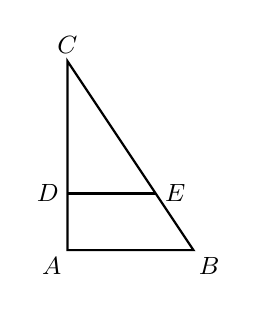
\begin{tikzpicture}[scale=0.8,font=\small]
\usetikzlibrary{calc}

\begin{scope}
%\clip (-2.1,-2.1) rectangle (2.5,2.1);
\coordinate (a) at (0,0);
\coordinate (b) at (2,0);
\coordinate (c) at (0,3);

\draw[thick] (a) node[shift={(-0.2,-0.2)}] {$A$} -- (b) node[shift={(0.2,-0.2)}] {$B$} -- (c) node[shift={(0,0.2)}] {$C$} -- cycle;

\draw[thick] ($(c)!0.7!(a)$) node[shift={(-0.25,0)}] {$D$} -- ($(c)!0.7!(b)$) node[shift={(0.25,0)}] {$E$};

\end{scope}


\end{tikzpicture}

%	\caption{Esercizio~\ref{ese:7.107}}\label{fig:ese7.107}
%\end{figure}
% \end{inaccessibleblock}

\begin{esercizio}[Giochi di Archimede 2005]
\label{ese:7.107}
Il triangolo $ABC$ è rettangolo ed i cateti $AB$ e $AC$ misurano 
rispettivamente 3~m e 4~m. Siano $B'$ e $C'$ punti appartenenti 
rispettivamente ai lati $AB$ e $AC$, tali che la retta contenente il 
segmento $B'C'$ sia parallela a quella contenete il segmento $BC$ e 
distante 1~m da essa. Calcolare l'area del triangolo $AB'C'$.
\end{esercizio}

%
% \begin{inaccessibleblock}[Figura: TODO]
%  \begin{figure}[!htb]
% 	\centering% Copyright (c) 2015 Daniele Masini - d.masini.it@gmail.com

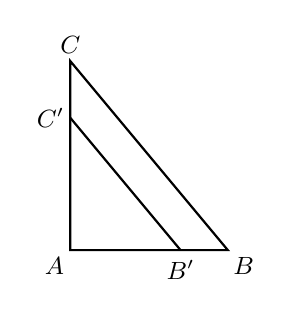
\begin{tikzpicture}[scale=0.8,font=\small]
\usetikzlibrary{calc}

\begin{scope}
%\clip (-2.1,-2.1) rectangle (2.5,2.1);
\coordinate (a) at (0,0);
\coordinate (b) at (2.5,0);
\coordinate (c) at (0,3);

\draw[thick] (a) node[shift={(-0.2,-0.2)}] {$A$} -- (b) node[shift={(0.2,-0.2)}] {$B$} -- (c) node[shift={(0,0.2)}] {$C$} -- cycle;

\draw[thick] ($(a)!0.7!(b)$) node[shift={(0,-0.25)}] {$B'$} -- ($(a)!0.7!(c)$) node[shift={(-0.25,0)}] {$C'$};

\end{scope}


\end{tikzpicture}

%	\caption{Esercizio~\ref{ese:7.108}}\label{fig:ese7.108}
%\end{figure}
% \end{inaccessibleblock}

\begin{esercizio}[Giochi d'Autunno 2011]
\label{ese:7.108}
L'area di un bosco, rappresentata dai vertici $F$, $O$, $I$ ed $N$, è 
un parallelogramma la cui base misura \np{1001}~m e la cui altezza 
misura \np{2012}~m. Il punto $S$ si trova sulla base $NI$ a 143~m dal 
vertice $I$. Qual è l'area del quadrilatero $BOIS$?
\end{esercizio}

%
% \begin{inaccessibleblock}[Figura: TODO]
%  \begin{figure}[!htb]
% 	\centering% Copyright (c) 2015 Daniele Masini - d.masini.it@gmail.com

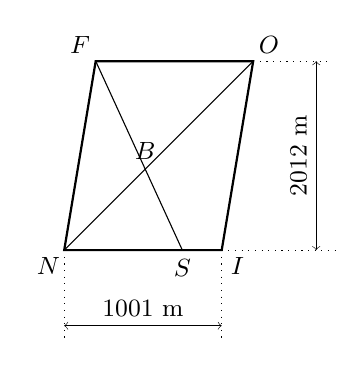
\begin{tikzpicture}[scale=0.8,font=\small]
\usetikzlibrary{calc}

\begin{scope}
%\clip (-2.1,-2.1) rectangle (2.5,2.1);
\coordinate (a) at (0,0);
\coordinate (b) at (2.5,0);
\coordinate (c) at (3,3);
\coordinate (d) at (0.5,3);

\draw[thick] (a) node[shift={(-0.2,-0.2)}] {$N$} -- (b) node[shift={(0.2,-0.2)}] {$I$} -- (c) node[shift={(0.2,0.2)}] {$O$} -- (d) node[shift={(-0.2,0.2)}] {$F$} -- cycle;

\draw[very thin, <->] (0,-1.2) coordinate (n1) -- node[above] {1001 m} (2.5,-1.2) coordinate (i1);
\draw[very thin, <->] (4,0) coordinate (i2) -- node[sloped,above] {2012 m} (4,3) coordinate (o2);

\draw[dotted] (c) -- ($(c)!1.2!(o2)$);
\draw[dotted] (b) -- ($(b)!1.2!(i2)$);
\draw[dotted] (a) -- ($(a)!1.2!(n1)$);
\draw[dotted] (b) -- ($(b)!1.2!(i1)$);

\draw (d) -- ($(a)!0.75!(b)$) coordinate (s) node[below] {$S$};
\draw (a) -- (c);
\coordinate (r) at (intersection of d--s and a--c);
\node[above] at (r) {$B$};

\end{scope}


\end{tikzpicture}

%	\caption{Esercizio~\ref{ese:7.109}}\label{fig:ese7.109}
%\end{figure}
% \end{inaccessibleblock}

\begin{esercizio}[Giochi d'Autunno 2011]
\label{ese:7.109}
Nel parallelogramma $ABCD$ il segmento $BD$ è perpendicolare ad $AB$ 
ed $E$ e $F$ sono i punti medi di $AB$ e $CD$ rispettivamente. 
Calcolare l'area del quadrilatero $GEHF$, sapendo che $AB=5$~cm e 
$BD=2$~cm.
\end{esercizio}

%
% \begin{inaccessibleblock}[Figura: TODO]
%  \begin{figure}[!htb]
% 	\centering% Copyright (c) 2015 Daniele Masini - d.masini.it@gmail.com

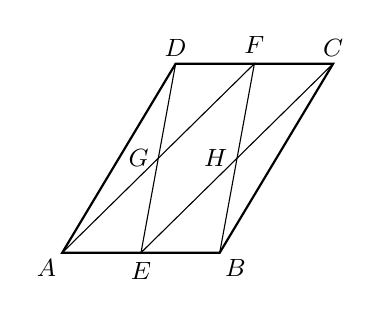
\begin{tikzpicture}[scale=0.8,font=\small]
\usetikzlibrary{calc}

\begin{scope}
\coordinate (a) at (0,0);
\coordinate (b) at (2.5,0);
\coordinate (c) at (4.3,3);
\coordinate (d) at (1.8,3);
\coordinate (e) at ($(a)!0.5!(b)$);
\coordinate (f) at ($(c)!0.5!(d)$);

\draw[thick] (a) node[shift={(-0.2,-0.2)}] {$A$} -- (b) node[shift={(0.2,-0.2)}] {$B$} -- (c) node[shift={(0,0.2)}] {$C$} -- (d) node[shift={(0,0.2)}] {$D$} -- cycle;

\draw (a) -- (f) -- (b);
\draw (c) -- (e) -- (d);

\coordinate (h) at (intersection of e--c and f--b);
\coordinate (g) at (intersection of d--e and a--f);

\node[above] at (f) {$F$};
\node[below] at (e) {$E$};

\node[left] at (g) {$G$};
\node[left] at (h) {$H$};

\end{scope}


\end{tikzpicture}

%	\caption{Esercizio~\ref{ese:7.110}}\label{fig:ese7.110}
%\end{figure}
% \end{inaccessibleblock}

\begin{esercizio}[Giochi d'Autunno 2010]
\label{ese:7.110}
In un triangolo due angoli misurano rispettivamente $30\grado$ e 
$105\grado$ ed il lato tra essi compreso è lungo 2~cm. Qual è la 
misura del perimetro del triangolo? 
\end{esercizio}

\begin{esercizio}[Giochi d'Autunno 2011]
\label{ese:7.111}
In un parallelogramma di area 1~m\textsuperscript{2} le lunghezze di 
due lati consecutivi sono una il doppio dell'altra. Inoltre uno degli 
angoli interni misura $60\grado$. Quanto misura la diagonale minore?
\end{esercizio}

\begin{esercizio}[Giochi d'Autunno 2010]
\label{ese:7.112}
In un triangolo equilatero $ABC$ con lato di lunghezza 3~m, prendiamo 
i punti $D$, $E$ e $F$ sui lati $AC$, $AB$ e $BC$ rispettivamente, in 
modo che i segmenti $AD$ e $FC$ misurino 1~m e il segmento $DE$ sia 
perpendicolare ad $AC$. Quanto misura l'area del triangolo $DEF$?
\end{esercizio}

%
% \begin{inaccessibleblock}[Figura: TODO]
%  \begin{figure}[!htb]
% 	\centering% Copyright (c) 2015 Daniele Masini - d.masini.it@gmail.com

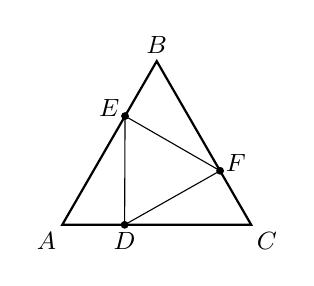
\begin{tikzpicture}[scale=1.2,font=\small]
\usetikzlibrary{calc}

\begin{scope}
\draw[thick] (0,0) coordinate (a) node[shift={(-0.2,-0.2)}] {$A$} -- ++(0:2) coordinate (c) node[shift={(0.2,-0.2)}] {$C$} -- ++(120:2) coordinate (b) node[shift={(0,0.2)}] {$B$} -- cycle;

\coordinate (d) at ($(a)!0.33!(c)$);
\coordinate (f) at ($(c)!0.33!(b)$);
\path (d) let \p1 = (d) in -- ({\x1},{\y1+1}) coordinate (d1);
\coordinate (e) at (intersection of d--d1 and a--b);

\draw (d) -- (e) -- (f) -- cycle;

\draw[fill] (d) circle (1pt) node[shift={(0,-0.2)}] {$D$};
\draw[fill] (e) circle (1pt) node[shift={(-0.2,0.1)}] {$E$};
\draw[fill] (f) circle (1pt) node[shift={(0.2,0.1)}] {$F$};

\end{scope}


\end{tikzpicture}

%	\caption{Esercizio~\ref{ese:7.113}}\label{fig:ese7.113}
%\end{figure}
% \end{inaccessibleblock}

\begin{esercizio}[Giochi di Archimede 2005]
\label{ese:7.113}
Dato un quadrato $ABCD$ si uniscono i punti medi dei lati aventi un 
vertice in comune formando un nuovo quadrato $EFGH$. Ripetiamo la 
stessa operazione per $EFGH$ e otteniamo un nuovo quadrato 
$A'B'C'D'$. Quanto vale il rapporto tra l'area di $ABCD$ e l'area di 
$A'B'C'D'$?
\end{esercizio}

\end{multicols}


\subsection{Risposte}

\begingroup
\hypersetup{linkcolor=black}

\paragraph{\ref{ese:7.10}.}
$25/4$~cm.

\paragraph{\ref{ese:7.11}.}
18~cm.

\paragraph{\ref{ese:7.12}.}
$24a^2$.

\paragraph{\ref{ese:7.13}.}
135~cm\textsuperscript{2}.

\paragraph{\ref{ese:7.14}.}
$2p=96a$,\quad $A=93/2a^2$.

\paragraph{\ref{ese:7.15}.}
$AH=20$~cm,\quad $2p=\np{220,1}$~cm.

\paragraph{\ref{ese:7.16}.}
$A=4\sqrt{3}a^2$,\quad $d_1=2\sqrt{3}a$,\quad $d_2=2\sqrt{7}a$.

\paragraph{\ref{ese:7.17}.}
$2p=50a$,\quad $A=150a^2$.

\paragraph{\ref{ese:7.18}.}
$2p=10a(2\sqrt{3}+3)/3$,\quad $A=25a^2/\sqrt{3}$.

\paragraph{\ref{ese:7.19}.}
34~cm,\quad 12~cm.

\paragraph{\ref{ese:7.20}.}
$\frac{3}{4}\sqrt{3}$~m\textsuperscript{2}.

\paragraph{\ref{ese:7.21}.}
$2+\sqrt{6}$~cm\textsuperscript{2}.

\paragraph{\ref{ese:7.22}.}
$2p=28+5(\sqrt{6}+\sqrt{10})$~cm.

\paragraph{\ref{ese:7.23}.}
$4+2/\sqrt{3}$,\quad $4\sqrt{3}+2$.

\paragraph{\ref{ese:7.24}.}
$6+2\sqrt{3}$.

\paragraph{\ref{ese:7.25}.}
$18(1+\sqrt{3})$,\quad $27(4+\sqrt{3})$.

\paragraph{\ref{ese:7.26}.}
$28+8\sqrt{2}$,\quad $80$.

\paragraph{\ref{ese:7.27}.}
$10(1+\sqrt{2})$,\quad $25$.

\paragraph{\ref{ese:7.28}.}
$24(9+\sqrt{3})$,\quad $36+12\sqrt{2}+12\sqrt{3}$.

\paragraph{\ref{ese:7.29}.}
$10+5\sqrt{34}$,\quad $\frac{125}{2}$.

\paragraph{\ref{ese:7.30}.}
$14\sqrt{2}+8\sqrt{6}$,\quad $14\sqrt{3}+24$.

\paragraph{\ref{ese:7.31}.}
$EH=EK=4$~m,\quad $2p=8(\sqrt{3}+1)$~m,\quad $C=8\pi$.

\paragraph{\ref{ese:7.32}.}
a)~$2p=2x(\sqrt{2}+3)$; $A=4x^2$,\quad b)~$2p=2x(4+\sqrt{3})$; 
$A=2x^2(1+\sqrt{3})$,\quad c)~$2p=2x(2+\sqrt{3})$; 
$A=2x^2(3+\sqrt{3})$.

\paragraph{\ref{ese:7.33}.}
$\frac{11}{6}a\sqrt{2}+a\sqrt{6}$,\quad $\frac{1}{6}a^2(e+2\sqrt{3})$.

\paragraph{\ref{ese:7.34}.}
$2p=a+3a\sqrt{3}$,\quad $A=\frac{1}{2}a^2\sqrt{3}$.

\paragraph{\ref{ese:7.35}.}
$6a\sqrt{3}+9a$,\quad $\frac{1}{24}(21a^2\sqrt{3}+36a^2)$.

\paragraph{\ref{ese:7.36}.}
$2\sqrt[4]{27}$~m.

\paragraph{\ref{ese:7.37}.}
$4\sqrt{2}$.

\paragraph{\ref{ese:7.40}.}
$16/9$.

\paragraph{\ref{ese:7.41}.}
$3/4$.

\paragraph{\ref{ese:7.42}.}
36,\quad 18.

\paragraph{\ref{ese:7.43}.}
12~cm\textsuperscript{2},\quad 12~cm\textsuperscript{2},\quad 
$172\grado$.

\paragraph{\ref{ese:7.44}.}
$\np{0,665}$,\quad $\np{10,85}$~cm.

\paragraph{\ref{ese:7.45}.}
$\np{300,12}$~mm.

\paragraph{\ref{ese:7.46}.}
36,\quad $\np{0,625}$.

\paragraph{\ref{ese:7.48}.}
42~cm,\quad 108~cm\textsuperscript{2},\quad $\np{7,2}$~cm.

\paragraph{\ref{ese:7.49}.}
$\np{11,25}$~cm\textsuperscript{2},\quad 
$\np{5,625}$~cm\textsuperscript{2}.

\paragraph{\ref{ese:7.50}.}
$252$~cm\textsuperscript{2}.

\paragraph{\ref{ese:7.51}.}
3~cm,\quad 6~cm\textsuperscript{2},\quad $\np{2,4}$~cm,\quad 
5~cm,\quad $\np{3,5}$~cm.

\paragraph{\ref{ese:7.52}.}
100~cm.

\paragraph{\ref{ese:7.53}.}
$\np{33,59}$~cm\textsuperscript{2}.

\paragraph{\ref{ese:7.54}.}
$\np{15,48}$~cm\textsuperscript{2}.

\paragraph{\ref{ese:7.57}.}
$45\grado$,\quad $67,5\grado$.

$\np{42,24}$~cm\textsuperscript{2}.

\paragraph{\ref{ese:7.59}.}
180~cm\textsuperscript{2}.

\paragraph{\ref{ese:7.61}.}
$176\grado13'30''$,\quad $50\grado21'$,\quad $40\grado16'48''$.

\paragraph{\ref{ese:7.62}.}
$\np{1080}$~cm\textsuperscript{2}.

\paragraph{\ref{ese:7.63}.}
384~cm\textsuperscript{2},\quad 80~cm.

\paragraph{\ref{ese:7.64}.}
328~cm,\quad $\np{2880}$~cm\textsuperscript{2},\quad $\np{35,15}$~cm.

\paragraph{\ref{ese:7.65}.}
250~cm\textsuperscript{2}.

\paragraph{\ref{ese:7.66}.}
768~cm\textsuperscript{2},\quad 40~cm.

\paragraph{\ref{ese:7.68}.}
$\np{1500}$~cm\textsuperscript{2},\quad 65~cm.

\paragraph{\ref{ese:7.69}.}
$\np{49,5}$~cm\textsuperscript{2}.

\paragraph{\ref{ese:7.70}.}
200~cm,\quad $\np{2304}$~cm\textsuperscript{2}.

\paragraph{\ref{ese:7.71}.}
84~cm\textsuperscript{2},\quad 252~cm\textsuperscript{2}.

\paragraph{\ref{ese:7.77}.}
40~cm.

\paragraph{\ref{ese:7.79}.}
$54\sqrt{7}$~cm\textsuperscript{2},\quad 
$84\sqrt{7}$~cm\textsuperscript{2}.

\paragraph{\ref{ese:7.83}.}
224~m,\quad 238~m,\quad $\np{23520}$~m\textsuperscript{2}.

\paragraph{\ref{ese:7.84}.}
6~cm,\quad 10~cm,\quad 8~cm.

\paragraph{\ref{ese:7.85}.}
80~cm,\quad 300~cm\textsuperscript{2}.

\paragraph{\ref{ese:7.87}.}
$14 + 2\sqrt{3}$~cm.

\paragraph{\ref{ese:7.89}.}
$9 + 5\sqrt{3} + 2\sqrt{7}$~cm,\quad 
$29\sqrt{3}/2$~cm\textsuperscript{2}.

\paragraph{\ref{ese:7.91}.}
$\np{30,2}$,\quad $\np{53,75}$.

\paragraph{\ref{ese:7.92}.}
$\np{22,4}$; $\np{19,5}$.

\paragraph{\ref{ese:7.93}.}
$A=14$.

\paragraph{\ref{ese:7.95}.}
$D(-4;2)$.

\paragraph{\ref{ese:7.99}.}
12~cm.

\endgroup
